\newpage
\section{Experimentos y Análisis de Resultados}
\label{sec:experimentos}

\subsection{Configuración Experimental y Parámetros}

Para evitar redundancias, se remite al Punto \ref{sec:formulacion} para la definición formal del problema, los conjuntos de datos (IBEX 35, S\&P 100 y S\&P 500) y las restricciones sobre las posiciones de los activos. A continuación se especifican los detalles experimentales necesarios para la reproducibilidad y la comparación empírica.

\subsubsection*{Condiciones de ejecución}

\begin{itemize}
    \item \textbf{Ejecuciones independientes:} 50 por algoritmo y mercado. Semilla base $seed=42$, incrementada secuencialmente ($42+i$).
    \item \textbf{Criterio de parada global:} máximo de 10\,000 evaluaciones de la función objetivo para todos los algoritmos estocásticos.
    \item \textbf{Datos y partición temporal:} fase de búsqueda de optimización en el periodo 2015--2024 y fase de prueba de dicha optimización en el periodo 2025 para todos los algoritmos.
\end{itemize}

\subsubsection*{Parámetros de los algoritmos de trayectoria}

\begin{itemize}
    \item \textbf{Enfriamiento Simulado:} $\mu=0.2$, $\phi=0.3$, $T_f=10^{-3}$, $max\_vecinos=10 \cdot n$ y $max\_exitos = n$ (equivalente a $0.1\cdot max\_vecinos$).
    \item \textbf{BMB e ILS:} 5 arranques por ejecución. La BL interna se acota a 2000 evaluaciones por arranque.
    \item \textbf{ILS:} tasa de mutación del 20\% para la perturbación de la mejor solución.
    \item \textbf{ILS-ES:} misma perturbación que ILS, sustituyendo la BL por ES en cada arranque.
\end{itemize}

\subsubsection*{Parámetros de la búsqueda local en el algoritmo de referencia (P2)}

El mejor algoritmo de la Práctica 2 identificado en las ejecuciones es \textbf{AM-Best}. Se mantiene como referencia en tablas y análisis con los parámetros configurados en \texttt{config.cfg}:

\begin{itemize}
    \item \textbf{Frecuencia:} cada 10 generaciones.
    \item \textbf{Aplicación:} BL aplicada al 10\% superior (AM-Best).
    \item \textbf{Intensidad:} máximo 100 evaluaciones por BL; ratio de transferencia reducido al 15\%.
\end{itemize}

\subsection{Resultados Numéricos y Boxplots}

Se muestran las tablas exigidas por el guion, incluyendo Greedy, Random y BL (P1), el mejor algoritmo de P2 (AM-Best), y las técnicas de trayectoria de P3 (BMB, ILS, ES, ILS-ES). Los valores provienen de la salida de ejecución en \texttt{salida.txt}.

\begin{table}[H]
\centering
\caption{Resultados numéricos -- IBEX 35}
\label{tab:global-ibex35}
\resizebox{\textwidth}{!}{%
\begin{tabular}{lcccccc}
\hline
Algoritmo & Fitness(2015--2024) & Fitness(2025) & Beneficio(2025) & Std & Evaluaciones & Tiempo (s) \\
\hline
Greedy & -4.794 & -3.227 & -0.033 & 0.000 & 1 & 0.000 \\
Random & -4.911 & -3.305 & 0.052 & 0.091 & 10000 & 0.025 \\
BL & -4.614 & -3.116 & 0.021 & 0.039 & 1078 & 0.001 \\
Mejor P2 (AM-Best) & -4.490 & -3.083 & 0.033 & 0.000 & 10000 & 0.007 \\
BMB & -4.574 & -3.107 & 0.023 & 0.020 & 5403 & 0.004 \\
ILS & -4.606 & -3.115 & 0.021 & 0.036 & 4349 & 0.003 \\
ES & -4.653 & -3.126 & 0.020 & 0.010 & 3244 & 0.002 \\
ILS-ES & -4.649 & -3.127 & 0.020 & 0.014 & 3130 & 0.002 \\
\hline
\end{tabular}
}
\end{table}

\begin{table}[H]
\centering
\caption{Resultados numéricos -- S\&P 100}
\label{tab:global-sp100}
\resizebox{\textwidth}{!}{%
\begin{tabular}{lcccccc}
\hline
Algoritmo & Fitness(2015--2024) & Fitness(2025) & Beneficio(2025) & Std & Evaluaciones & Tiempo (s) \\
\hline
Greedy & -3.305 & -3.791 & 0.100 & 0.000 & 1 & 0.000 \\
Random & -3.400 & -4.080 & 0.079 & 0.041 & 10000 & 0.069 \\
BL & -3.116 & -3.890 & 0.097 & 0.084 & 4351 & 0.023 \\
Mejor P2 (AM-Best) & -2.816 & -3.734 & 0.100 & 0.008 & 10000 & 0.036 \\
BMB & -3.006 & -3.863 & 0.092 & 0.046 & 10000 & 0.065 \\
ILS & -3.114 & -3.888 & 0.097 & 0.082 & 9926 & 0.055 \\
ES & -3.300 & -3.987 & 0.088 & 0.030 & 1828 & 0.011 \\
ILS-ES & -3.311 & -3.991 & 0.085 & 0.038 & 2863 & 0.017 \\
\hline
\end{tabular}
}
\end{table}

\begin{table}[H]
\centering
\caption{Resultados numéricos -- S\&P 500}
\label{tab:global-sp500}
\resizebox{\textwidth}{!}{%
\begin{tabular}{lcccccc}
\hline
Algoritmo & Fitness(2015--2024) & Fitness(2025) & Beneficio(2025) & Std & Evaluaciones & Tiempo (s) \\
\hline
Greedy & -3.370 & -3.909 & 0.024 & 0.000 & 1 & 0.000 \\
Random & -3.648 & -4.364 & 0.019 & 0.044 & 10000 & 0.678 \\
BL & -3.428 & -4.330 & 0.004 & 0.154 & 9645 & 0.603 \\
Mejor P2 (AM-Best) & -2.735 & -3.898 & 0.017 & 0.037 & 10000 & 0.367 \\
BMB & -3.263 & -4.189 & 0.010 & 0.078 & 10000 & 1.071 \\
ILS & -3.434 & -4.312 & 0.005 & 0.146 & 10000 & 0.689 \\
ES & -4.062 & -4.760 & 0.010 & 0.101 & 308 & 0.016 \\
ILS-ES & -4.035 & -4.761 & 0.007 & 0.092 & 546 & 0.030 \\
\hline
\end{tabular}
}
\end{table}

A continuación se presentan los boxplots correspondientes a los algoritmos de la Práctica 3 para cada mercado:

\begin{figure}[H]
\centering
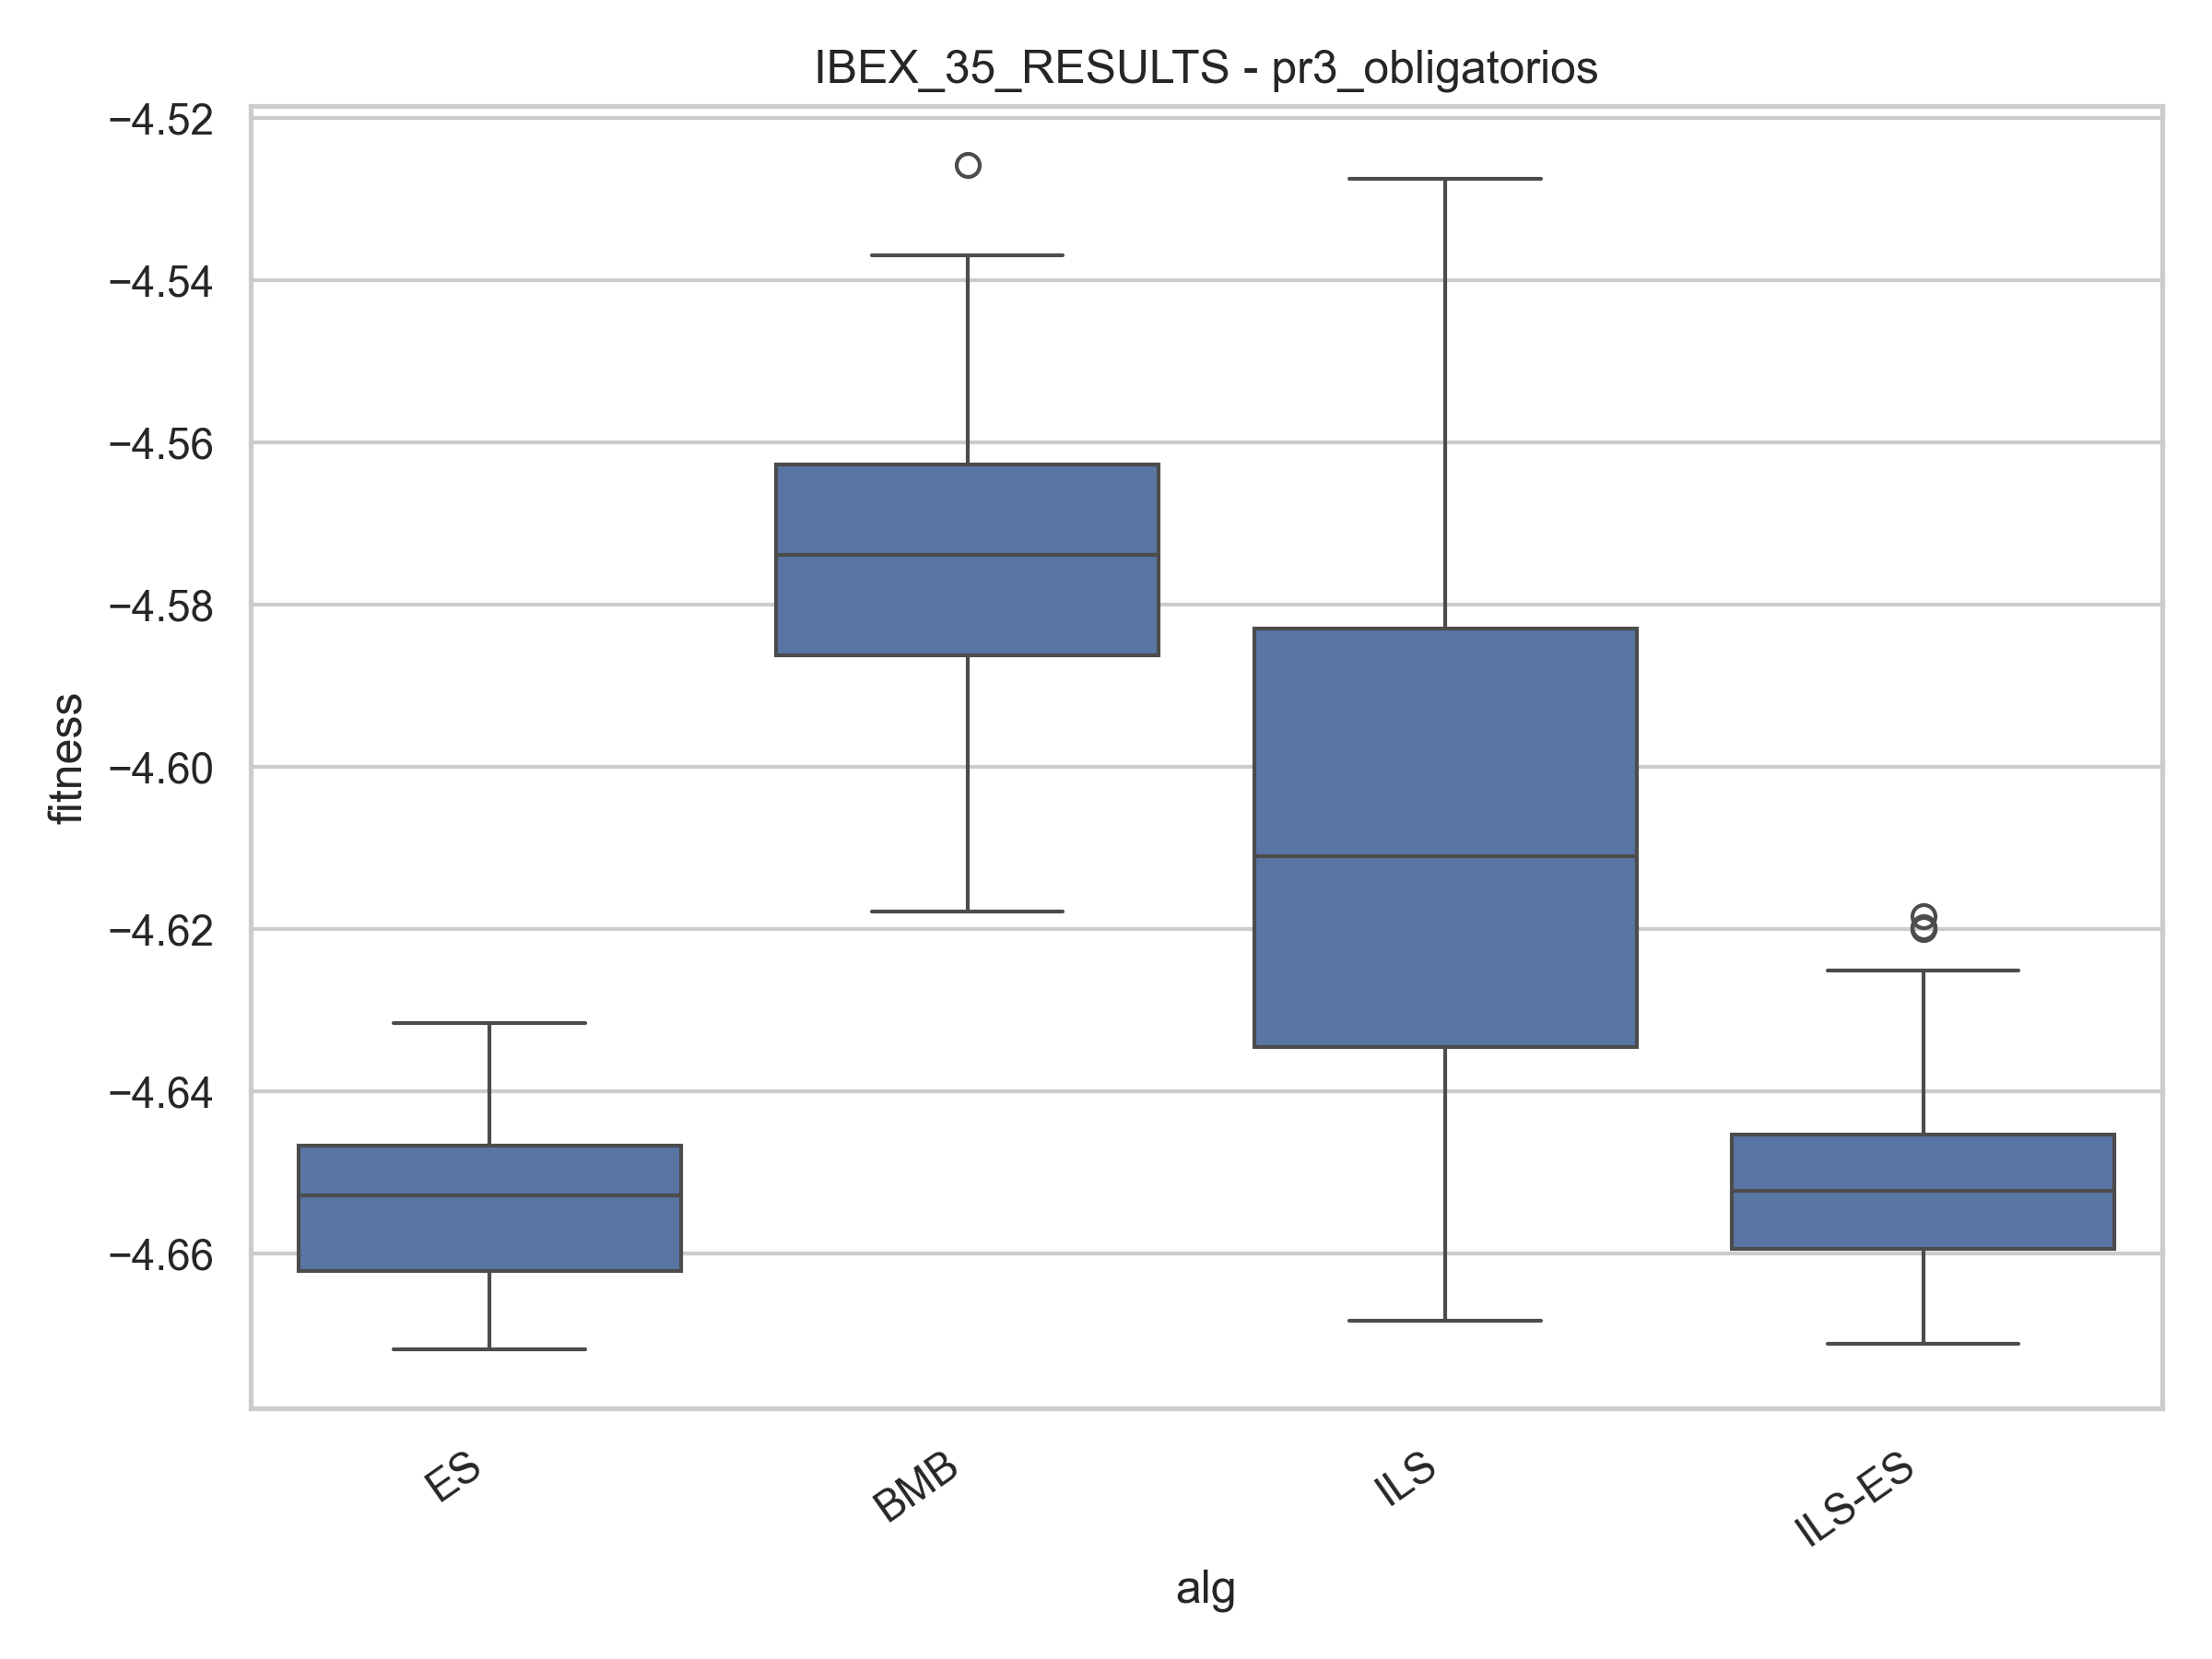
\includegraphics[width=0.8\textwidth]{figuras/IBEX_35_RESULTS_pr3_obligatorios.png}
\caption{Boxplots algoritmos trayectoria (Práctica 3) -- IBEX 35.}
\label{fig:pr3-obligatorios-ibex}
\end{figure}

\begin{figure}[H]
\centering

\includegraphics[width=0.8\textwidth]{\detokenize{figuras/S&P_100_RESULTS_pr3_obligatorios.png}}
\caption{Boxplots algoritmos trayectoria (Práctica 3) -- S\&P 100.}
\label{fig:pr3-obligatorios-sp100}
\end{figure}

\begin{figure}[H]
\centering

\includegraphics[width=0.8\textwidth]{\detokenize{figuras/S&P_500_RESULTS_pr3_obligatorios.png}}
\caption{Boxplots algoritmos trayectoria (Práctica 3) -- S\&P 500.}
\label{fig:pr3-obligatorios-sp500}
\end{figure}

\subsection{Análisis de Resultados}

El guion exige comparar algoritmos \textbf{similares} para aislar el elemento diferenciador.
La Figura~\ref{fig:heatmap-mejora} sintetiza en términos porcentuales la mejora (o empeoramiento)
de cada algoritmo respecto a la Búsqueda Local (BL), que actúa como referencia de partida.

\begin{figure}[H]
\centering
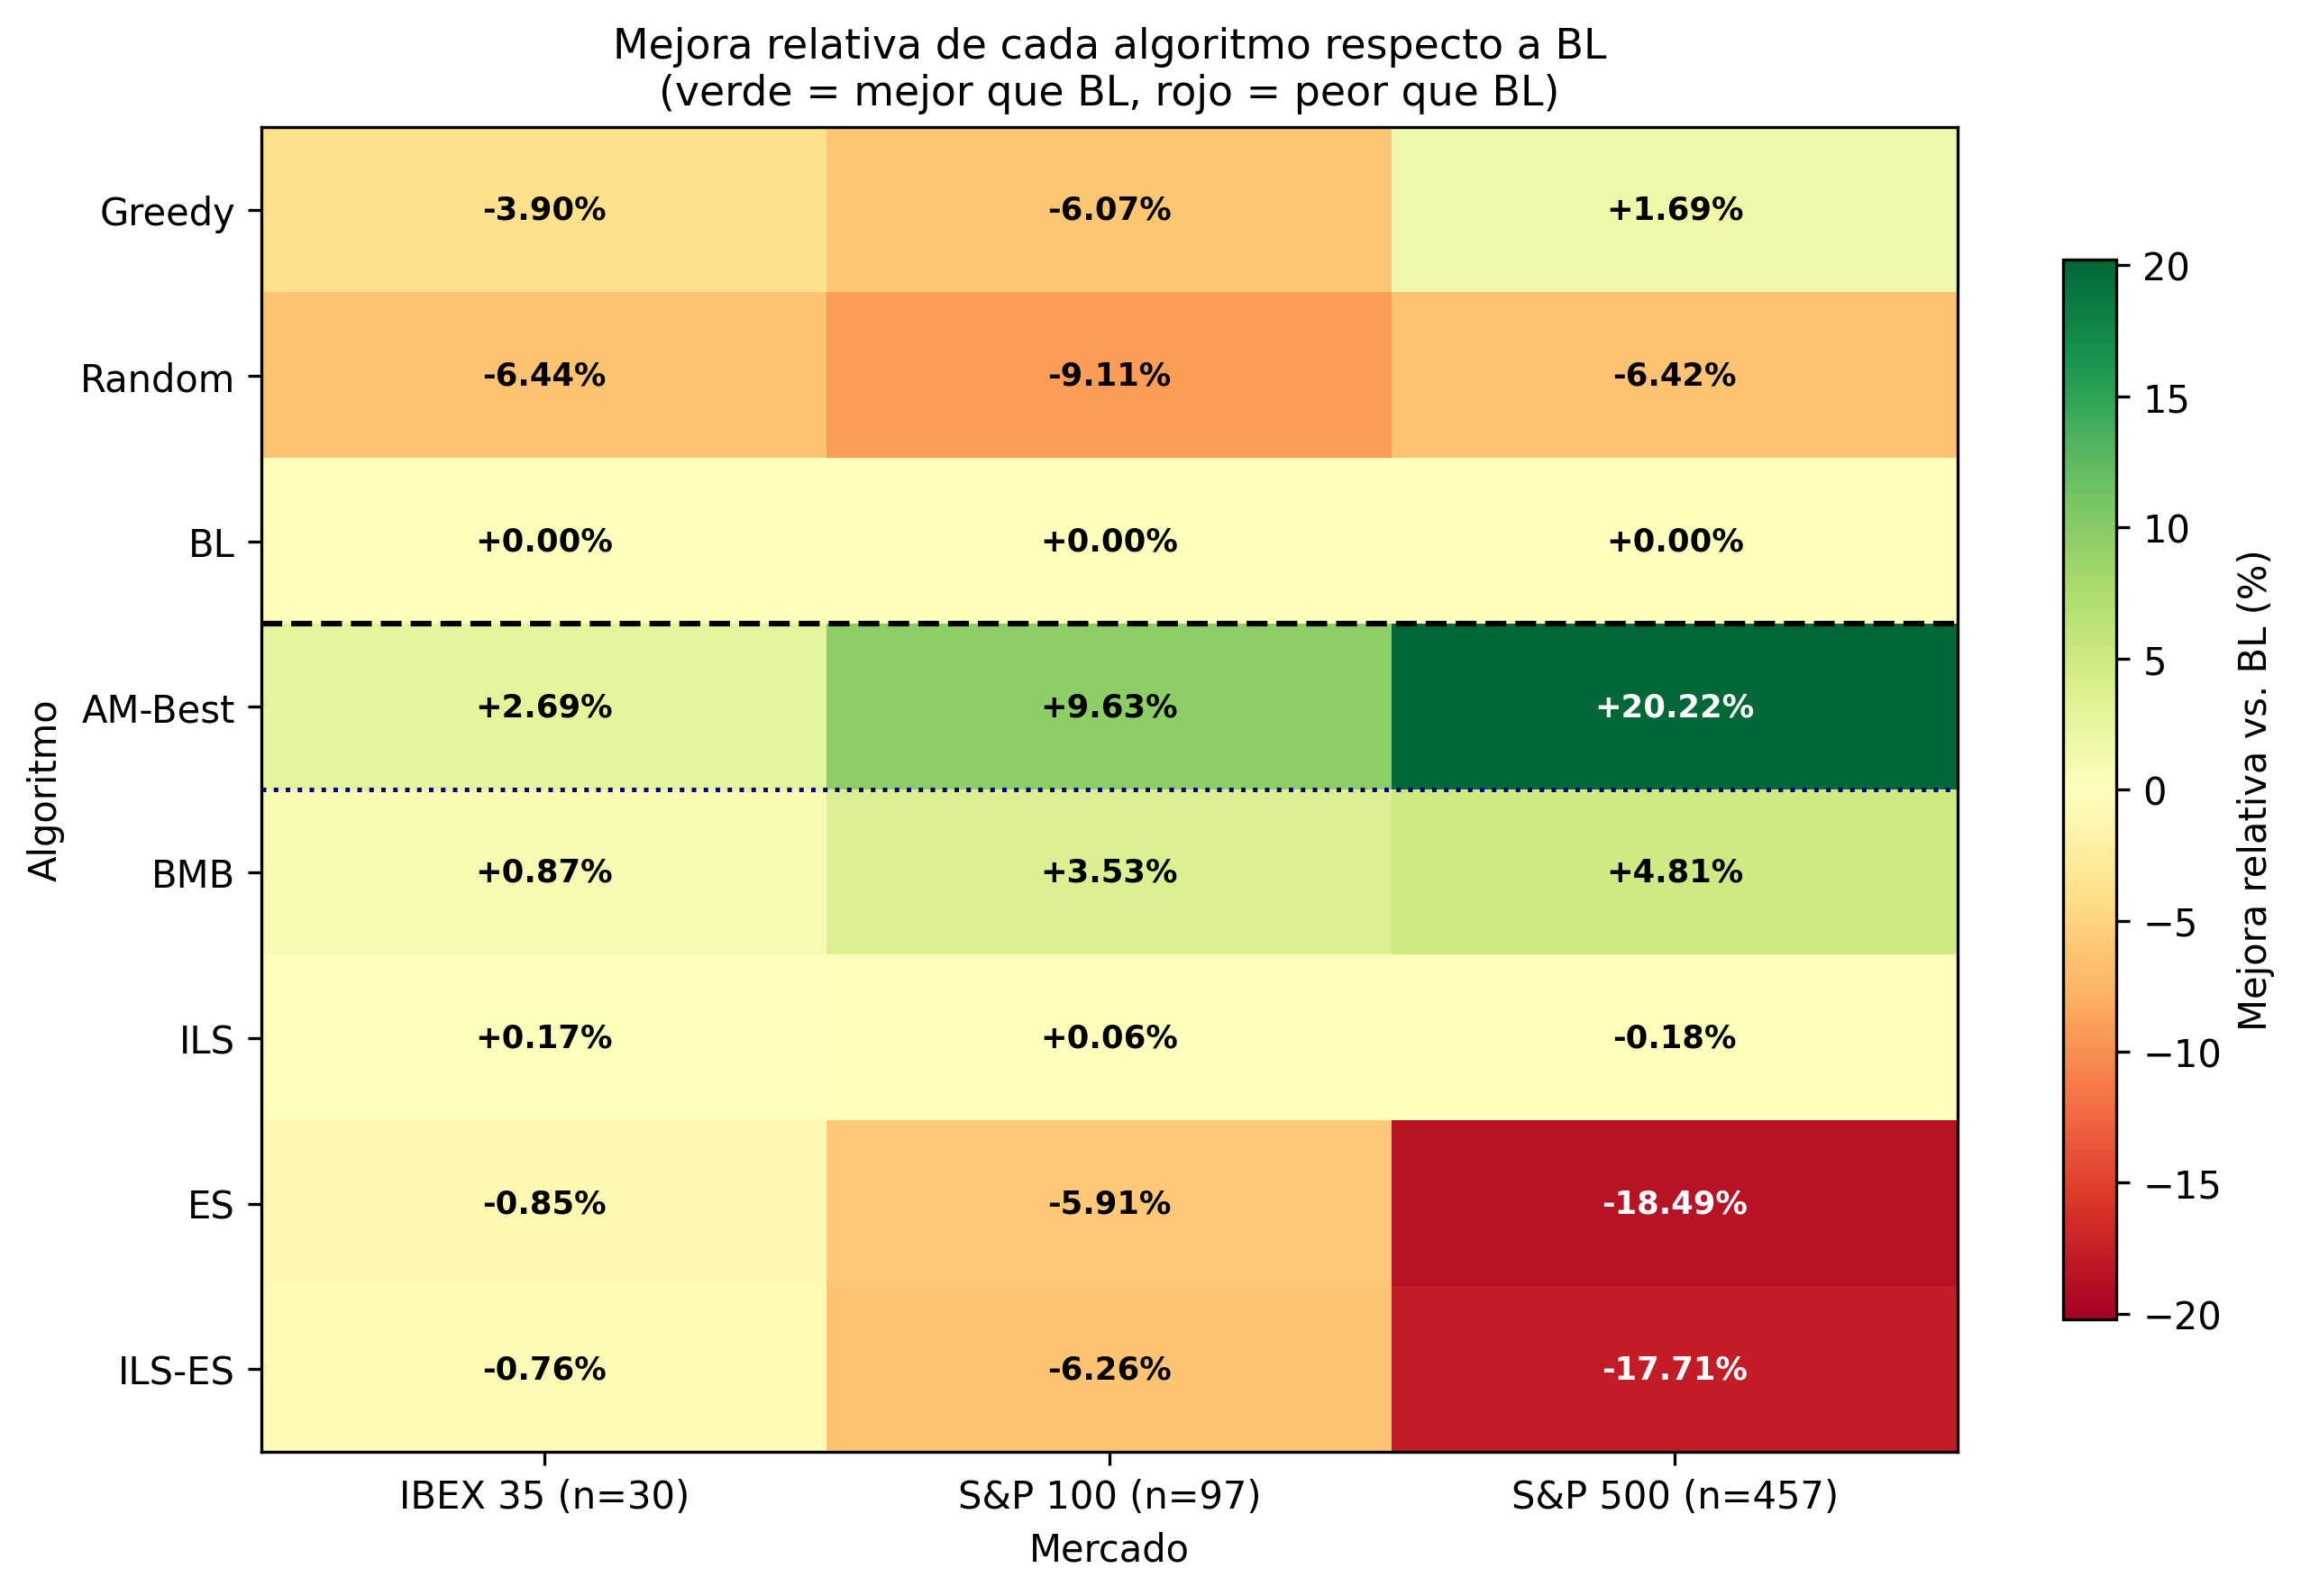
\includegraphics[width=\textwidth]{figuras/heatmap_mejora_vs_bl.png}
\caption{Mejora relativa porcentual de cada algoritmo respecto a BL.
Verde = supera a BL; rojo = peor que BL.}
\label{fig:heatmap-mejora}
\end{figure}


\subsubsection*{BL frente a las técnicas de trayectoria (BMB, ILS, ES, ILS-ES)}

La Búsqueda Local (BL) actúa como el punto de referencia y el bloque constituyente principal de los algoritmos BMB e ILS. Al analizar su rendimiento frente a las demás alternativas:

\textbf{BMB} demuestra ser sistemáticamente superior a BL, logrando mejoras del \textbf{+0.87\% en IBEX 35, +3.53\% en S\&P 100 y +4.81\% en S\&P 500}. Esta clara tendencia al alza a medida que aumenta la dimensión del problema se justifica teóricamente por la naturaleza explotadora de la BL. En un único arranque, la BL converge rápidamente al óptimo local de su cuenca de atracción inicial. BMB, al realizar 5 arranques aleatorios independientes con 2000 evaluaciones cada uno, consigue explorar múltiples regiones disjuntas del espacio de soluciones y seleccionar la mejor de ellas. Cuanto mayor es el espacio de búsqueda (especialmente en S\&P 500 con $N=457$ activos), más crítica resulta esta diversificación inicial para no quedar atrapado en cuencas de atracción de baja calidad.

\textbf{ILS} ofrece una mejora más modesta frente a BL, con un \textbf{+0.17\% en IBEX 35 y +0.06\% en S\&P 100}, mientras que en S\&P 500 experimenta un ligero retroceso del \textbf{-0.18\%}. Al contrario que BMB, ILS no realiza reinicios a ciegas, sino que aplica una perturbación del 20\% sobre la mejor solución actual. El hecho de que ILS sea menos efectivo que BMB en dimensiones altas revela que una mutación del 20\% no es lo suficientemente disruptiva en carteras grandes, provocando que la BL interna vuelva a caer reiteradamente en la misma cuenca de atracción o en cuencas adyacentes de similar calidad. Esto evidencia un exceso de explotación (búsqueda local muy concentrada) frente a la efectiva exploración global por reinicios aleatorios de BMB.

\textbf{ES} (Enfriamiento Simulado) obtiene resultados inferiores a la BL en todas las instancias: \textbf{-0.85\% en IBEX 35, -5.91\% en S\&P 100 y -18.49\% en S\&P 500}. La notable degradación de la calidad en S\&P 500 se debe a la parametrización interna y al presupuesto máximo de 10\,000 evaluaciones. Al fijarse $\max\_vecinos = 10N$ (4570 en S\&P 500) y $\max\_exitos = 1N$ (457), cada etapa de temperatura consume un volumen altísimo de evaluaciones. Esto restringe el número de enfriamientos térmicos $M$ a poco más de 2 ciclos antes de agotar el límite de 10\,000. Como consecuencia, el algoritmo finaliza prematuramente en fases de alta temperatura donde predomina la aceptación de movimientos desfavorables (comportamiento puramente exploratorio), sin presupuesto suficiente para la fase final de cristalización e intensificación hacia el óptimo local. Sin embargo, su coste temporal es extremadamente bajo (véanse las Figuras~\ref{fig:scatter-tradeoff-ibex}--\ref{fig:scatter-tradeoff-sp500}).

\subsubsection*{BMB frente a ILS: reinicio ciego vs. perturbación informada}

La comparación directa de estos dos métodos ilustra la tensión entre la diversificación radical y la intensificación con memoria. BMB supera a ILS en los tres conjuntos evaluados (ventaja neta de +0.70\% en IBEX 35, +3.47\% en S\&P 100 y +4.99\% en S\&P 500). En espacios de búsqueda reducidos (IBEX 35), la diferencia es pequeña porque las cuencas de atracción son pocas y fáciles de optimizar. No obstante, en el S\&P 500, la superioridad de BMB confirma que reiniciar la búsqueda desde 5 puntos del espacio geográficamente inconexos es una estrategia mucho más robusta para el problema de cartera que iterar sobre variaciones locales de una única solución base como hace ILS.

\subsubsection*{ES frente a ILS-ES: impacto de sustituir BL por ES como motor}

La hibridación ILS-ES sustituye la BL del ILS por el algoritmo de enfriamiento simulado como motor de optimización local. Comparado con la BL de referencia, ILS-ES obtiene pérdidas de calidad de \textbf{-0.76\% en IBEX 35, -6.26\% en S\&P 100 y -17.71\% en S\&P 500}. Aunque supera ligeramente a ES básico en todos los casos (por ejemplo, recuperando un +0.78\% de fitness relativo en S\&P 500), no logra igualar la calidad de ILS con BL. Esto confirma que el enfriamiento simulado, al estar limitado por el estricto presupuesto de evaluaciones, no actúa como un buen optimizador local de intensificación intermedia dentro de un esquema reiterado. Además, el criterio de Metrópolis propio de ES ya proporciona suficiente capacidad de escape ante óptimos locales, haciendo que el operador de perturbación externo de ILS resulte redundante y aporte escasa mejora.

\subsubsection*{AM-Best (P2) como referencia superior}

El algoritmo evolutivo memético con intensificación local selectiva (AM-Best) de la práctica anterior domina con rotundidad en todos los escenarios, logrando mejoras sobre BL del \textbf{+2.69\% en IBEX 35, +9.63\% en S\&P 100 y +20.22\% en S\&P 500}. La ventaja crece de manera exponencial con la dimensionalidad porque las aproximaciones poblacionales logran mantener y recombinar un conjunto diverso de soluciones de buena calidad. La aplicación selectiva de BL sobre el 10\% mejor de la población maximiza la eficiencia del presupuesto de evaluaciones, combinando de forma óptima la exploración a gran escala con la intensificación en regiones altamente prometedoras.


\subsubsection*{Análisis de outliers}

Los boxplots de las Figuras~\ref{fig:pr3-obligatorios-ibex}--\ref{fig:pr3-obligatorios-sp500}
muestran comportamientos atípicos que conviene justificar teóricamente:
\begin{itemize}[noitemsep]
    \item \textbf{IBEX 35 — outlier superior en BMB:} en una ejecución, el arranque aleatorio
    inicializó en una cuenca de atracción especialmente favorable; al no tener memoria del mejor
    anterior (como sí tiene ILS), ese arranque fue explotado hasta el máximo por la BL interna.
    \item \textbf{IBEX 35 — outliers superiores en ILS-ES:} la combinación del criterio de
    Metrópolis con la perturbación ILS permitió escapar de valles locales en dos ejecuciones
    concretas, saltando a cuencas de mayor calidad que no alcanzó ninguna otra técnica.
    \item \textbf{S\&P 100 — outlier inferior en BMB:} el punto de partida aleatorio cayó en
    una zona extremadamente pobre del espacio, y los 2000 evaluaciones de BL no fueron suficientes
    para escapar de ese valle.
    \item \textbf{S\&P 500 — outlier superior en ES:} en esa ejecución, el esquema de enfriamiento
    Cauchy modificado encontró por aceptación probabilística una cuenca de calidad inhabitual,
    demostrando que el criterio de Metrópolis puede —en ocasiones— superar a la explotación pura
    de BL incluso con muy pocas evaluaciones.
\end{itemize}

\subsection{Estudio de Eficiencia y Trade-off Calidad/Coste}

A continuación, se presentan de manera individualizada las gráficas que ilustran el compromiso
entre el fitness alcanzado y el tiempo computacional requerido para cada uno de los tres mercados
considerados (Figuras~\ref{fig:scatter-tradeoff-ibex}, \ref{fig:scatter-tradeoff-sp100} y
\ref{fig:scatter-tradeoff-sp500}).

\begin{figure}[H]
\centering
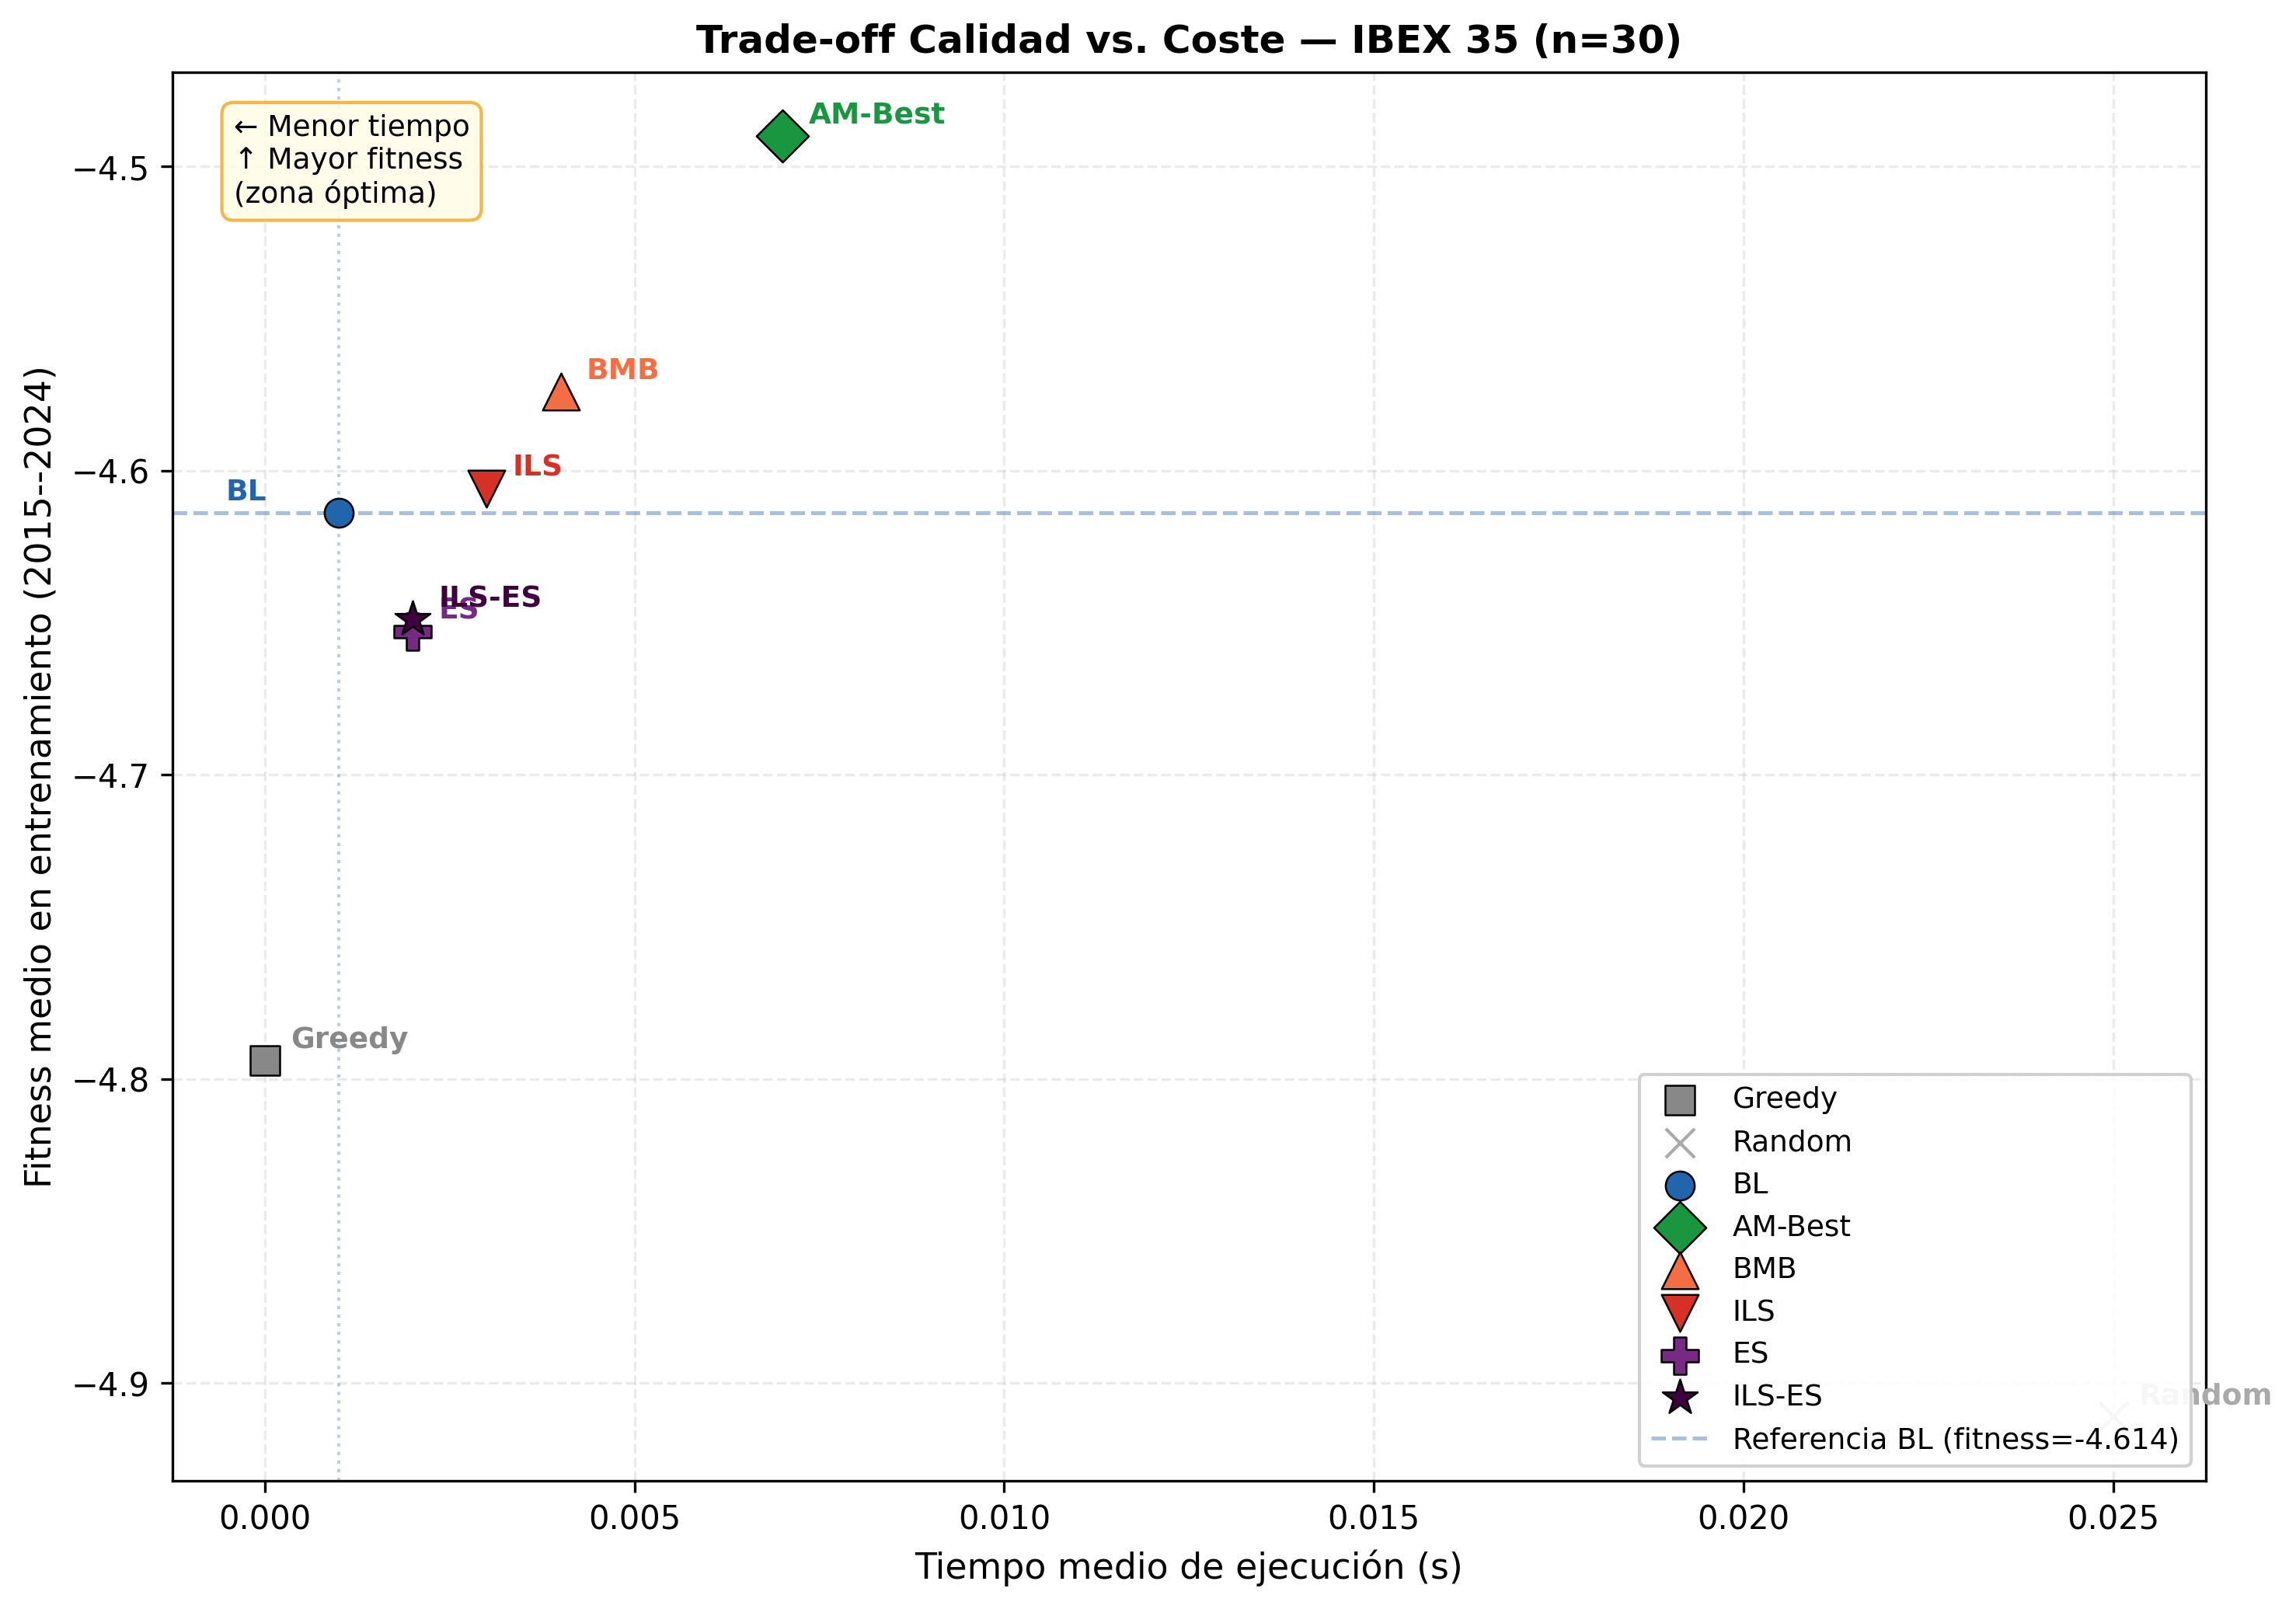
\includegraphics[width=0.85\textwidth]{figuras/scatter_tradeoff_ibex35.png}
\caption{Compromiso Calidad--Coste en el mercado IBEX 35 ($n=30$).}
\label{fig:scatter-tradeoff-ibex}
\end{figure}

\begin{figure}[H]
\centering
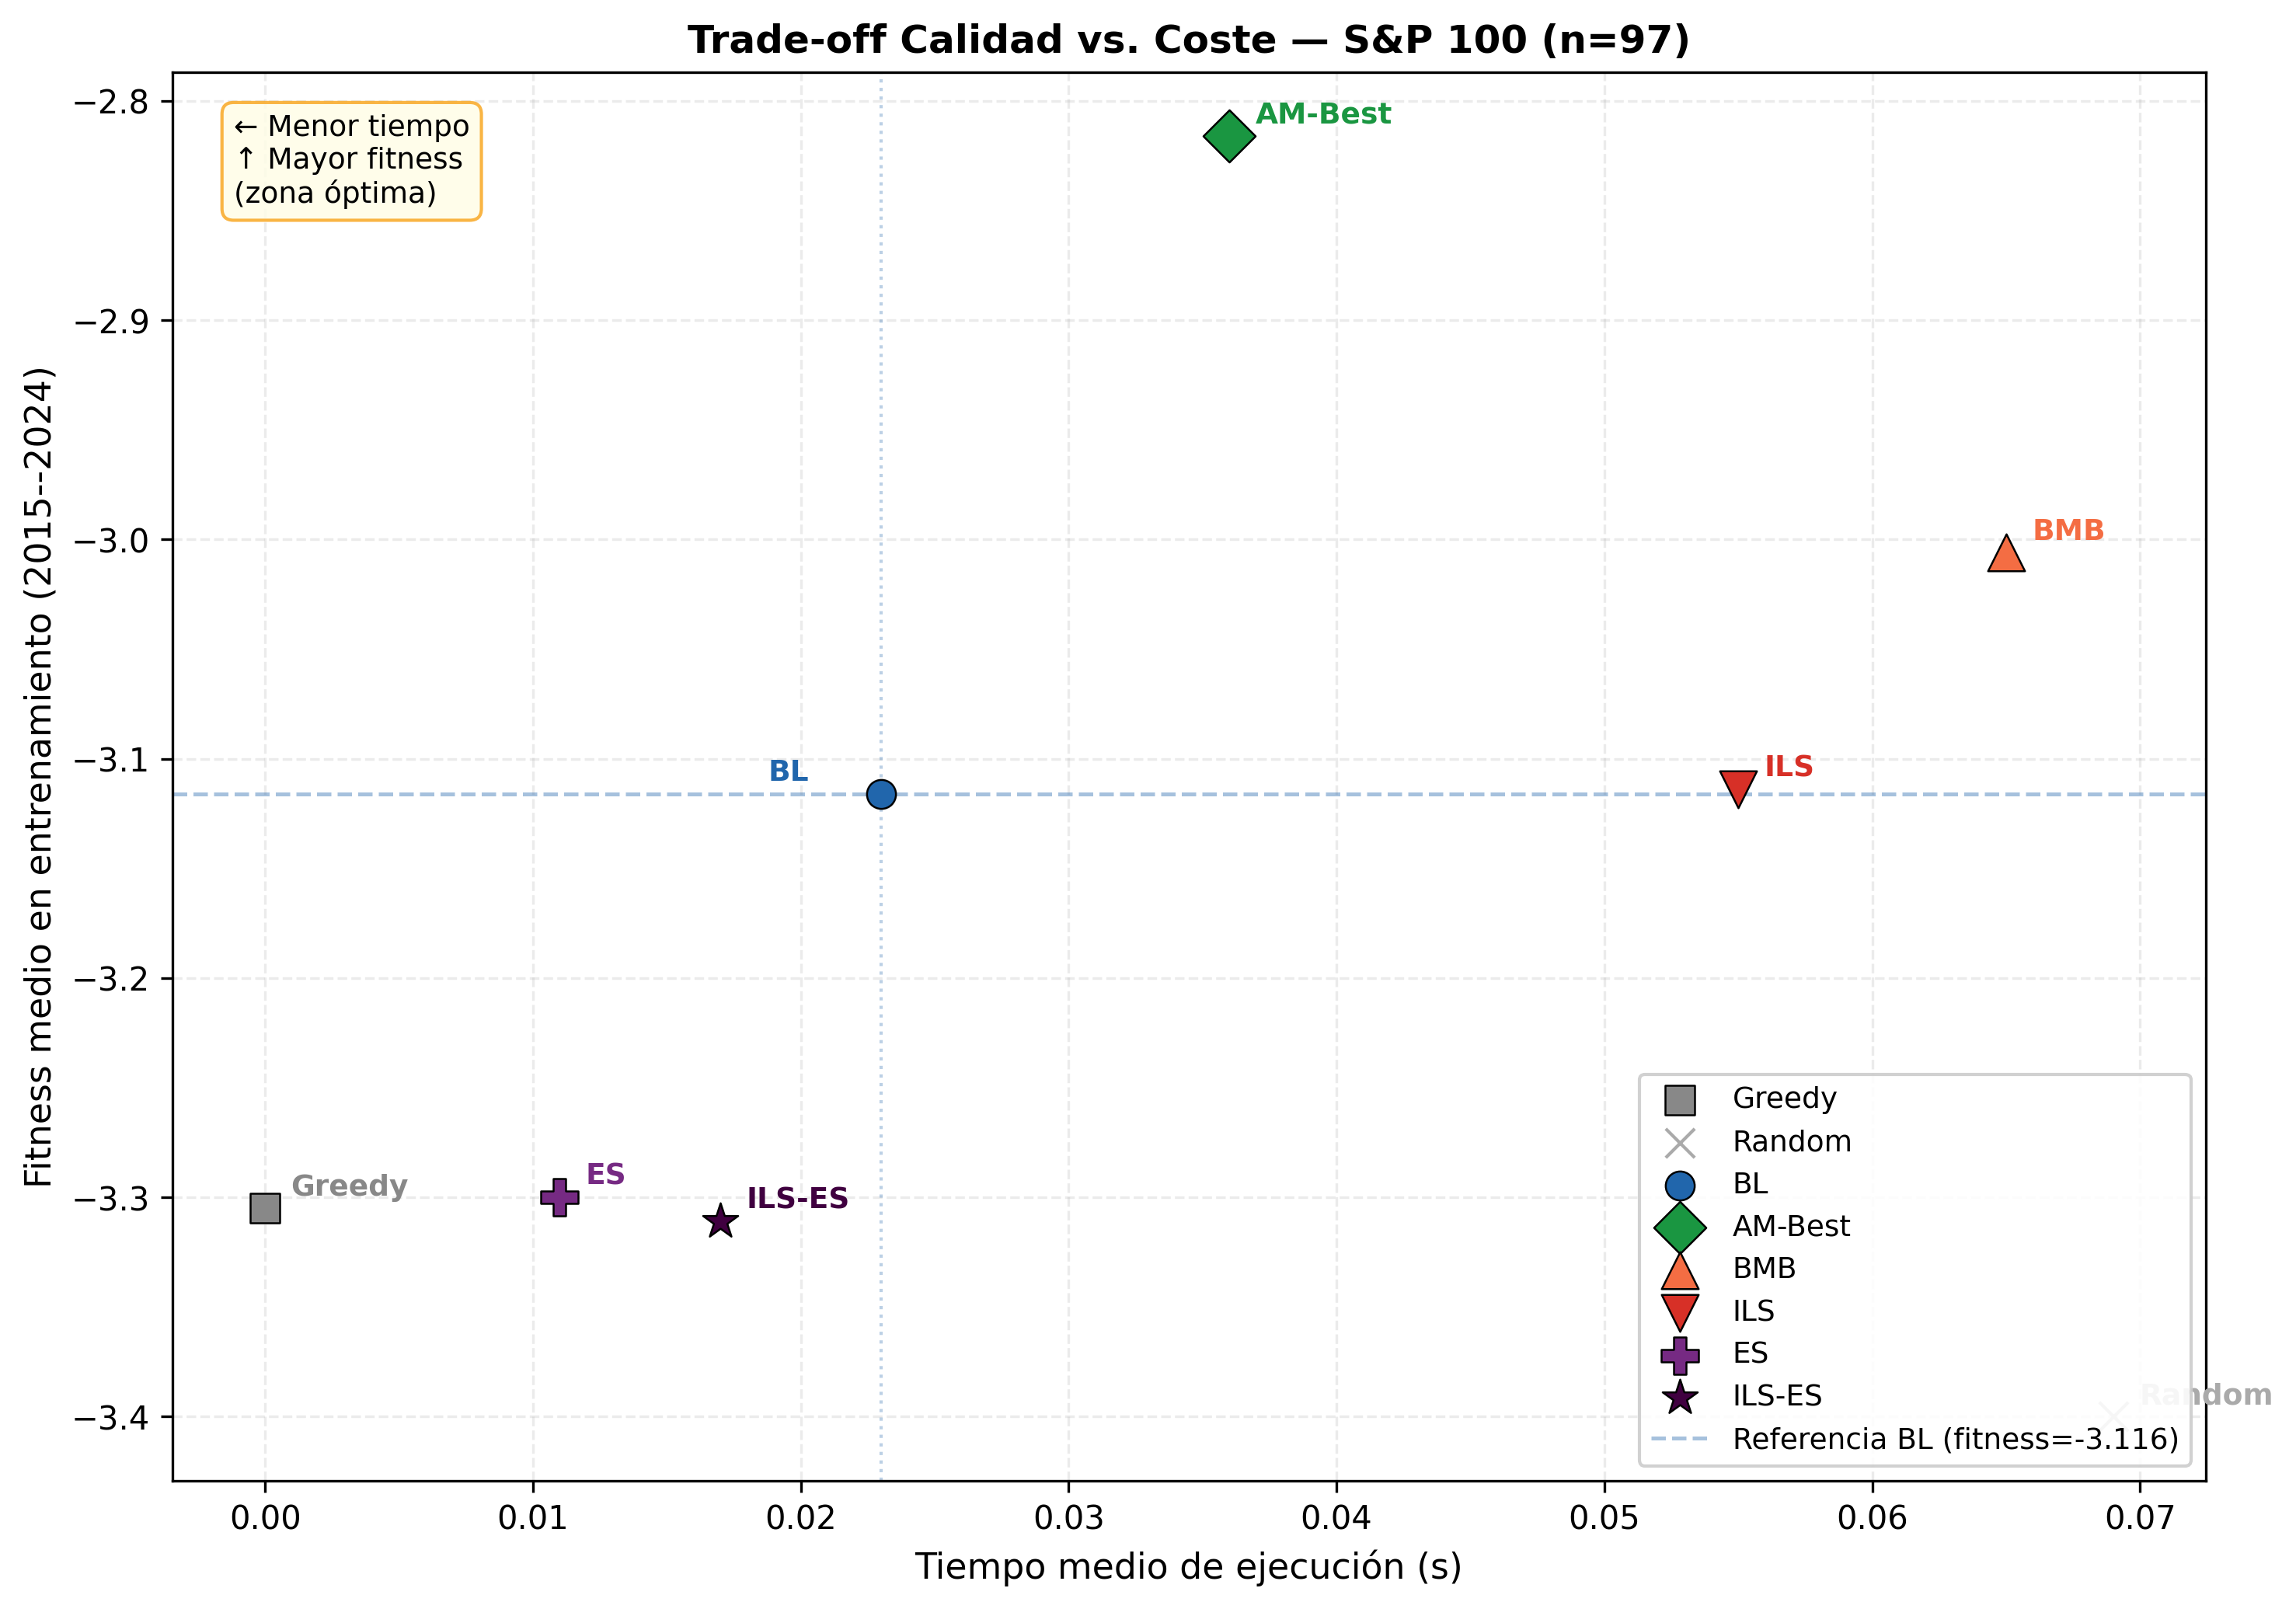
\includegraphics[width=0.85\textwidth]{figuras/scatter_tradeoff_sp100.png}
\caption{Compromiso Calidad--Coste en el mercado S\&P 100 ($n=97$).}
\label{fig:scatter-tradeoff-sp100}
\end{figure}

\begin{figure}[H]
\centering
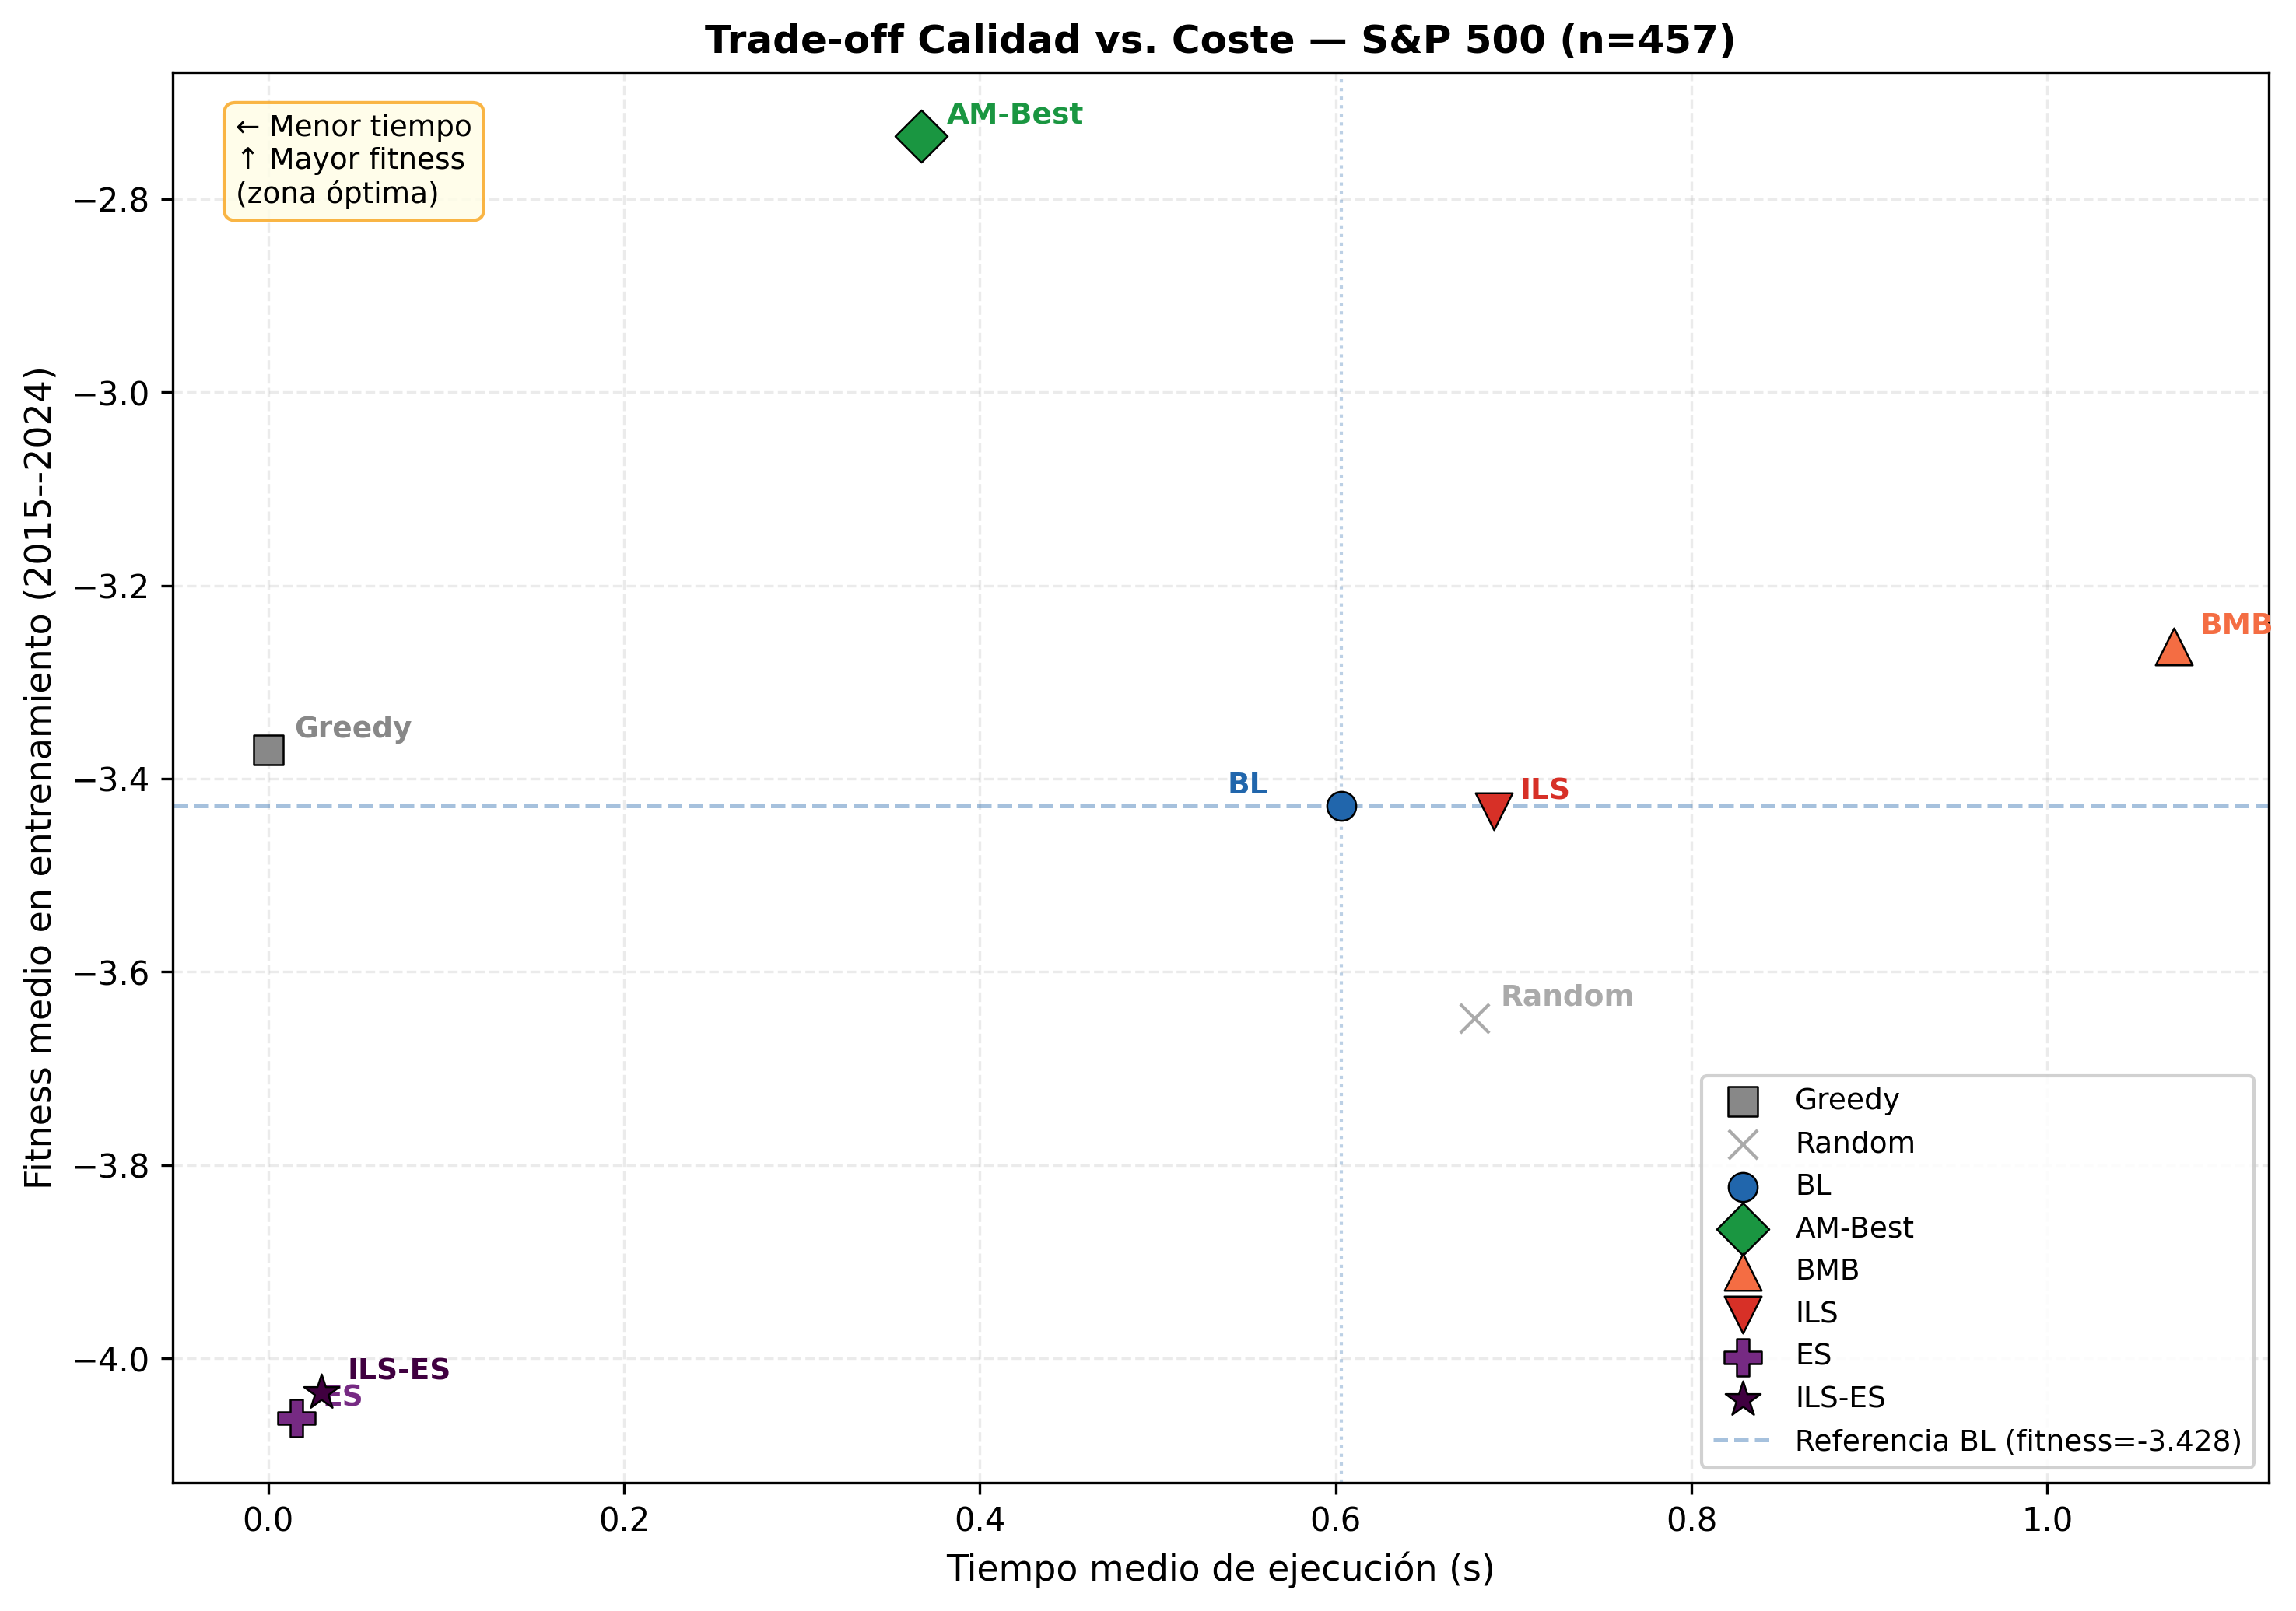
\includegraphics[width=0.85\textwidth]{figuras/scatter_tradeoff_sp500.png}
\caption{Compromiso Calidad--Coste en el mercado S\&P 500 ($n=457$).}
\label{fig:scatter-tradeoff-sp500}
\end{figure}

\begin{figure}[H]
\centering
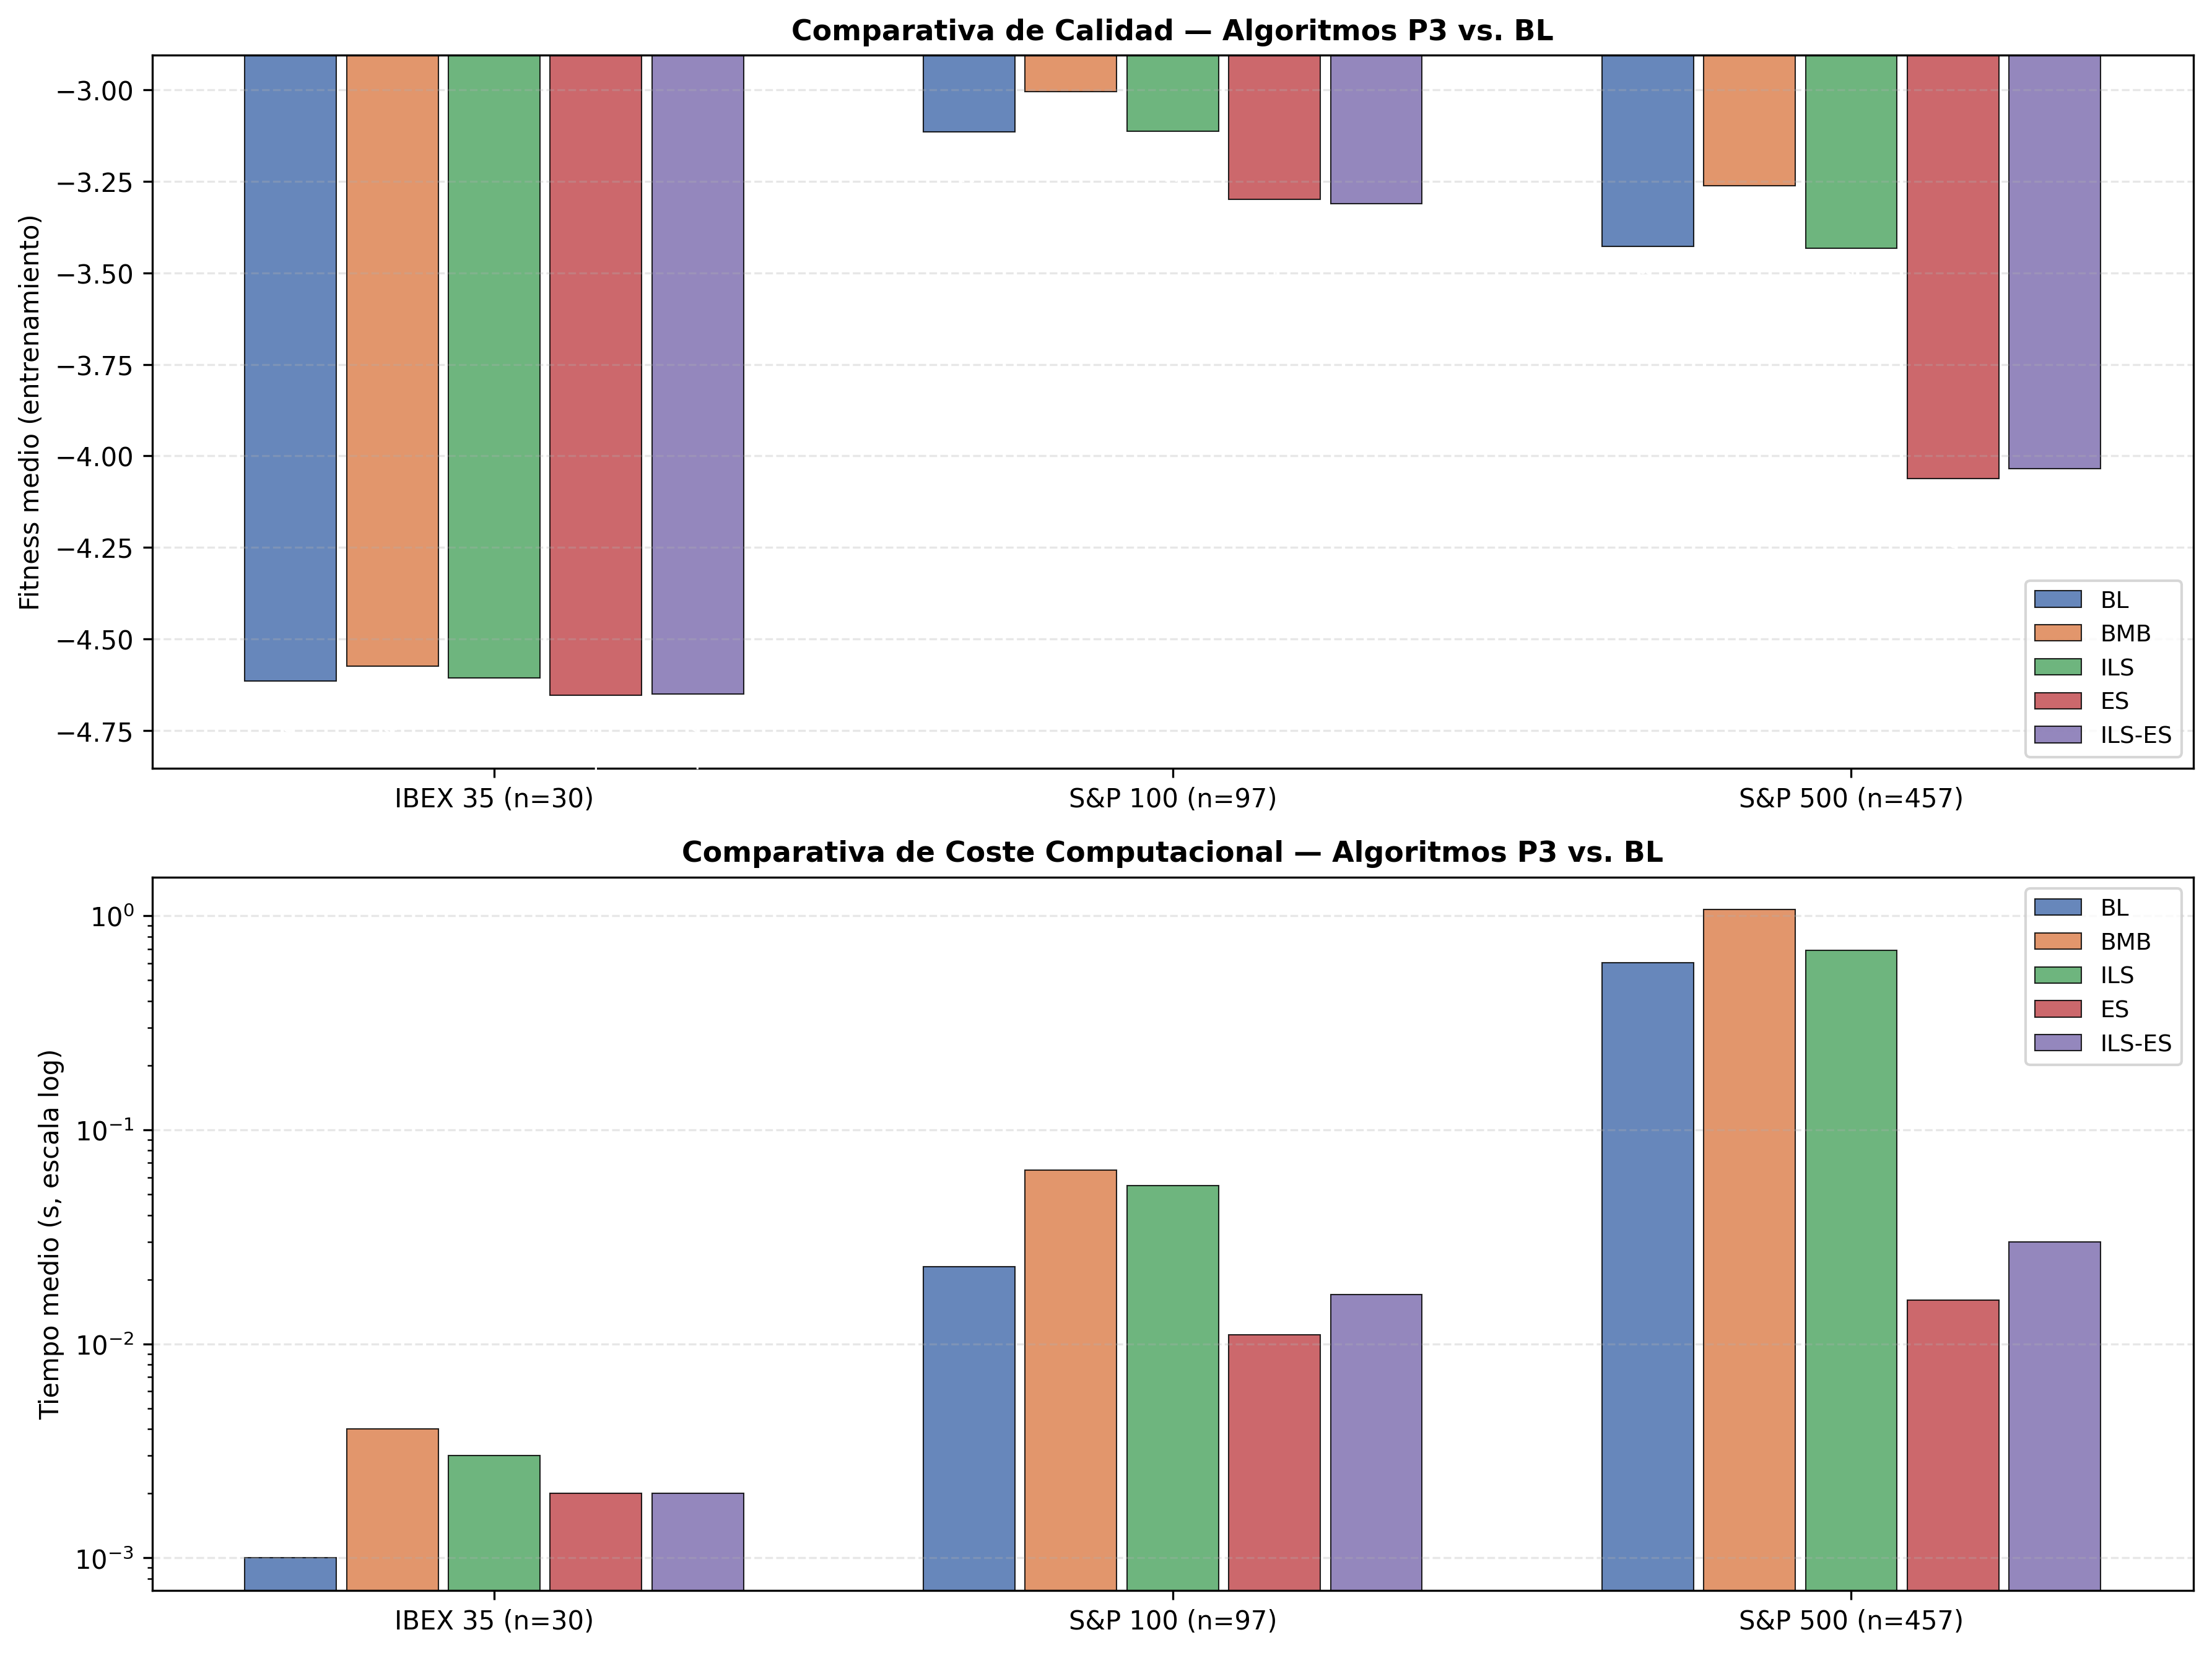
\includegraphics[width=0.9\textwidth]{figuras/barchart_p3_comparativa.png}
\caption{Comparativa directa de fitness (arriba) y tiempo en escala logarítmica (abajo)
para los algoritmos P3 y BL en los tres mercados.}
\label{fig:barchart-p3}
\end{figure}

Las Figuras~\ref{fig:scatter-tradeoff-ibex}--\ref{fig:scatter-tradeoff-sp500} ilustran
con claridad el trade-off fundamental: ES e ILS-ES ocupan de forma sistemática la zona de
\textit{bajo tiempo y baja calidad} en dimensiones altas (como en el S\&P 500,
Figura~\ref{fig:scatter-tradeoff-sp500}), mientras que BMB e ILS se desplazan hacia tiempos
mayores con calidad notablemente superior. Cabe destacar que el algoritmo Greedy se sitúa, en términos de coste temporal, por debajo de ILS-ES y ES en el IBEX 35, y a un nivel muy similar en el S\&P 100 debido a su naturaleza constructiva directa. En IBEX 35 (Figura~\ref{fig:scatter-tradeoff-ibex}),
debido a la reducida escala del problema, todos los algoritmos de P3 se agrupan en un rango de coste
mínimo ($<0.01$ s), por lo que BMB resulta la opción preferible al ofrecer la mejor calidad
relativa sin penalización temporal apreciable.

La Figura~\ref{fig:barchart-p3} confirma en escala logarítmica que \textbf{ES e ILS-ES son
entre 3$\times$ y 40$\times$ más rápidos que BMB e ILS} en S\&P 500, pagando ese coste con
una reducción de calidad de aproximadamente el $18\%$ respecto a BL. Este trade-off clásico
intensificación-coste justifica la coexistencia de técnicas de trayectoria simple (ES) y múltiple
(BMB, ILS): dependiendo de los requisitos específicos de la aplicación práctica (optimización en
tiempo real versus planificación estratégica), resultará adecuado emplear un enfoque u otro. Además, en el caso específico del IBEX 35, la Búsqueda Local (BL) es la técnica iterativa de optimización que menos tiempo consume, convergiendo casi instantáneamente.



